
\section{Konzepte von Optimierungsverfahren für nichtlineare Modelle}
Während dieser Vorlesungsreihe beleuchten wir die Thematik physikalische Größen zu ermitteln, die
indirekt zugänglich sind. Sie werden über eine Modellbildung als Modellparameter approximiert.
In den bisherigen Kapiteln hatten wir uns damit befasst, Modellparameter linearer Modelle, zu schätzen.
Die Besonderheit dabei ist, dass die \textsl{Kostenfunktion} $Q$ eine lineare Abhängigkeit von den
Modellparametern hat, so dass die Modellparameter
im Fall der Ausgleichsrechnung nach der Methode der kleinsten Quadrate durch Lösen eines 
linearen Gleichungssystems ermittelt werden können.
Im vorangegangen Kapitel wurde in Gl.~(\ref{linRegGleichungssystem}), Gl.~(\ref{GleichungssytemKostenfkt})
 und Gl.~(\ref{LsgRegressionGlSys}) gezeigt, dass das Gleichungssystem
aufgestellt wird, indem der Gradient, der die Kostenfunktion nach den Modellparametern ableitet, gleich Null
gesetzt wird, um das Maximum zu finden.

Für den Fall, dass die Modellparameter nicht linear in die Kostenfunktion $Q$,
auch \textsl{Zielfunktional} genannt, eingehen,
erfolgt die Schätzung der Modellparameter durch Variation, also durch Optimierung derart, um
das Minimum der Optimierungszielfunktion $Q$ zu finden.

Wir sind von normalverteilten Abweichungen ausgegangen und haben uns
die Likelihoodverteilungen angeschaut. Als Beispiel nehmen wir ein Modell mit 2 Parametern, bei
dem eine Gerade durch den Ursprung des Koordinatensystems eines dreidimensionalen
Raums gehe und bei dem alle drei Achsen von der gleichen physikalischen Dimension seien.
Die beiden zu schätzenden Parameter seien hier der Azimutalwinkel $\alpha$ und der 
Polarwinkel $\theta$, die die gesuchte Richtung der Geraden beschreiben.
Ein Punkt $\mathbf{r}$, der exakt auf der Geraden liegt, erfülle
\begin{equation}
\mathbf{r} \; = \; \lambda \mathbf{u} \qquad \mathrm{mit} \qquad
\mathbf{u}(\alpha,\theta) \; = \; \left(\begin{array}{c}
\cos(\alpha) \sin(\theta)\\
\sin(\alpha) \sin(\theta)\\
\cos(\theta) \end{array}\right) \qquad \mathrm{und} \qquad \lambda \in I \!\! R.
\end{equation}
\begin{figure}
\begin{center}
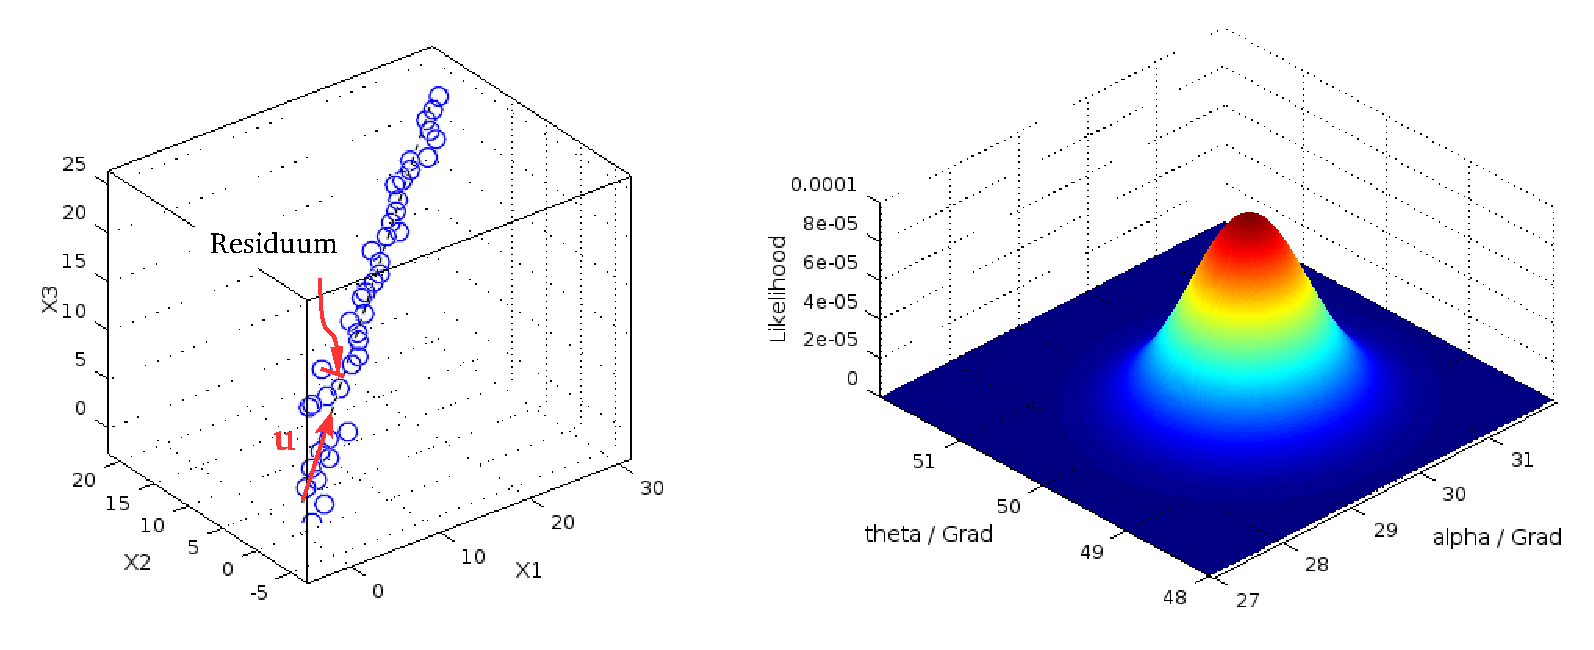
\includegraphics[width=0.95\textwidth, angle = 0]{03_vorlesung/media/LSopti_example1.pdf}
\end{center}
\caption{Modell mit 2 zu schätzenden Parametern (\textsl{links}) und der dazugehörigen
Likelihood für normalverteilte Residuen (\textsl{rechts}).\label{LSoptiExample1}}
\end{figure}

Abb.~\ref{LSoptiExample1} zeigt das Modell als schwarz gestrichelte Gerade und die Beobachtungen als blaue Kreise, sowie rechts die Likelihoodverteilung. Wir hatten bereits ausführlich darüber gesprochen, dass die Suche des Maximums der Likelihood in die Suche des Minimums übergeht. Es gelte nun diejenige Geradenrichtung zu finden, für die die senkrechten Abstände,
die Residuen $\varepsilon_j$,  der beobachteten Punkte (Messpunkte) $\mathbf{r}_{\mathrm{Mess},j} = (X_{1,j}, X_{2,j}, X_{3,j})^\mathsf{T}$ minimal sind. Für das Kriterium für minimale Abstände, also die Kostenfunktion $Q$, setzen wir wieder voraus, dass die Messpunkte gaußverteilt um eine Gerade streuen. Den Betrag für die senkrechten Abstände berechnen wir mit
\begin{equation}
\varepsilon(\alpha,\theta)_j \; = \; \left| \mathbf{r}_{\mathrm{Mess},j} \; - \;
( \mathbf{r}_{\mathrm{Mess},j} \cdot \mathbf{u}(\alpha,\theta) ) \, \mathbf{u}(\alpha,\theta) \right|
\end{equation}
mit $|$ als Betrag gemäß $| \mathrm{a} | = \sqrt{a_1^2 + a_2^2 + a_3^2}$.
Für die Likelihoodverteilung auf der rechten Seite von Abb.~\ref{LSoptiExample1} verwenden wir
die Wahrscheinlichkeitsdichte gemäß
\begin{equation}
p(\varepsilon_1,\dots,\varepsilon_J | \alpha, \theta)
\propto e^{-\frac{1}{2} \, \sum\limits_{j=1}^J \, \left(\frac{\varepsilon(\alpha,\theta)_j}{\sigma} \right)^2} .
\end{equation}
Für den Schätzvorgang wählen wir wieder für das Zielfunktional $Q$ die Summe der Quadrate der Residuen $Q = \sum \varepsilon_j^2$,
also einen Optimierungsvorgang gemäß der Methode der kleinsten
Residuenquadratsumme (RQS).
\begin{equation}
\min_{\alpha,\theta} \, \sum\limits_{j=1}^J \, \varepsilon(\alpha,\theta)_j^2 .
\end{equation}
Die Optimierungsrechnung bietet sehr unterschiedliche Methoden für eine Minimumsuche.

Wir können sie grob danach einteilen
\begin{itemize}
\item ob das nächste Modellparametertupel gemäß einer gewissen Strategie aus
mehreren Vor\-gänger\-tupeln mit den dazugehörigen Werten der Kostenfunktion $Q$ gewonnen wird
\item oder ob nicht nur die Kostenfunktion $Q$ direkt, sondern auch deren Gradienten bestimmt
werden.
\end{itemize}
Ein möglicher, vielfach genutzer Ansatz für das Verwenden mehrerer Vorgängertupel mit den dazugehörigen Werten der RQS
ist die Simplexmethode nach Nelder und Mead aus dem Jahr 1965. Er wird als Bibliotheksfunktion \texttt{fmins}
in Matlab und Gnu-Octave zur Verfügung gestellt. Mit Simplex ist ein Vieleck gemeint, das $M+1$ Ecken hat für $M$
Parameter, in unserem Beispiel also drei Ecken für zwei Parameter, was in Abb.~\ref{LSoptiExample1NM} durch
schwarz umrandete weiße Punkte, die mit schwarzen, durchgezogenen Linien verbunden sind, skizziert ist. Zum Aufbau eines
Startsimplex wird ein Startwerttupel $\mathbf{p}_{0,0}$ des Modellparametervektors gewählt und zu jedem Parameter ein
weiterer Vektor, der eine Variation $\Delta P_m$ repräsentiert:
\begin{equation}
\mathbf{p}_{0,1} \; = \; \mathbf{p}_{0,0} \; + \; \left(\begin{array}{c}
\Delta P_1 \\
0 \\
\vdots \\
0
\end{array}\right) \qquad
\mathbf{p}_{0,m} \; = \; \mathbf{p}_{0,0} \; + \; \left(\begin{array}{c}
0 \\
\vdots \\
0 \\
\Delta P_m \\
0 \\
\vdots \\
0
\end{array}\right) \qquad
\mathbf{p}_{0,M} \; = \; \mathbf{p}_{0,0} \; + \; \left(\begin{array}{c}
0 \\
\vdots \\
0 \\
\Delta P_M
\end{array}\right)
\end{equation}
\begin{figure}
\begin{center}
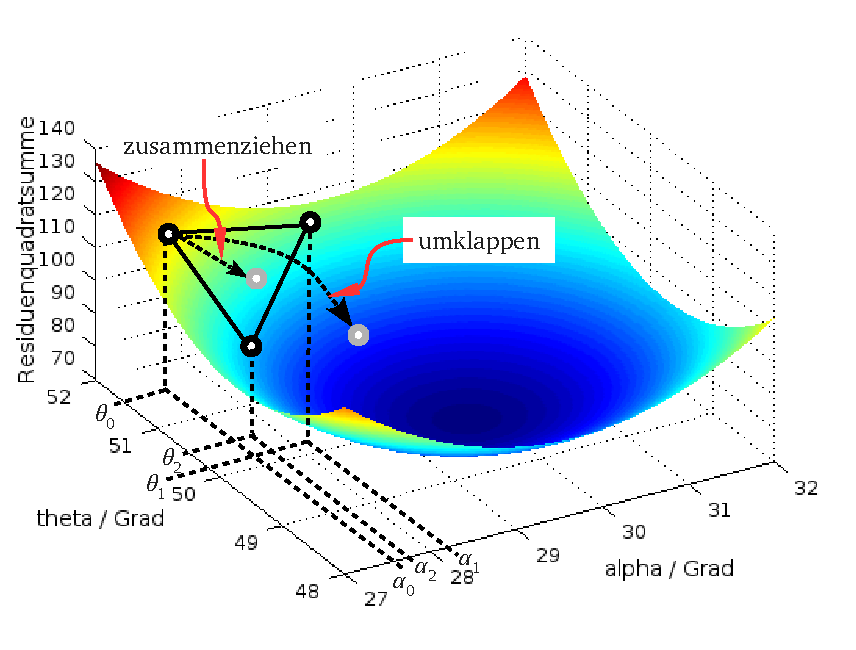
\includegraphics[width=0.6\textwidth, angle = 0]{03_vorlesung/media/LSopti_example1_LS_NM.pdf}
\end{center}
\caption{Residuenquadratsumme des Beispielmodells mit 2 zu schätzenden Parametern
und Simplex für Optimierungsverfahren nach Nelder und Mead.\label{LSoptiExample1NM}}
\end{figure}

Die Strategie ist es, diesen Simplex durch Zusammenziehen oder durch Umklappen dazu zu bewegen, in
die Minimumsmulde herunter zu klettern, was in Abb.~\ref{LSoptiExample1NM} durch hellgrau umrandete
weiße Punkte und durch Pfeile skizziert ist. Die Entscheidung, wann er sich zusammen zieht und dadurch
auch verkleinert und wann er umklappt und wann er notfalls auch wieder gestreckt (vergrößert) werden
muss wird anhand dessen getroffen, ob die Werte des Zielfunktionals $Q$ kleiner werden oder nicht.
Wenn er klein und flach im Tal angekommen ist, terminiert der Algorithmus. Hierzu gibt es dann noch
verschiedene Ansätze, wie überprüft wird, ob er zu weit über dem Tal waagerecht festhakt und eigentlich
noch eine zu große Mulde darunter liegt und eines der Simplexbeine angezogen werden muss.

Dieses Verfahren eignet sich auch für zu minimierende Zielfunktionale, die nicht so schön stetig
differenzierbar, d.h.\ glatt, in der Talmulde sind. Für Messungen mit Beobachtungen, die nicht gaußverteilt
streuen, sondern stark abweichende Punkte aufweisen, greift man auf andere Verteilungen zurück.
Eine mögliche Verteilung kann die Laplaceverteilung sein
\begin{equation}
p(\varepsilon_1,\dots,\varepsilon_J | \alpha, \theta)
\propto e^{-\frac{1}{2} \, \sum\limits_{j=1}^J \, \frac{| \varepsilon(\alpha,\theta)_j |}{\sigma} } 
\end{equation}
was bedeutet, dass sie eine Exponentialverteilung der Absolutbeträge der
Residuen ist. Bei dem zu minimierenden Exponenten
\begin{equation}
\min_{\alpha,\theta} \, \sum\limits_{j=1}^J \, | \varepsilon(\alpha,\theta)_j |
\end{equation}
bildet sich die Minimumsmulde durch die Betragsbildung zu einer ausgeprägt scharfen Spitze aus.
Im Minimum gibt es also keine einheitliche Steigung. Je nach Richtung, von der man sich ihr nähert,
gibt es sehr unterschiedliche Steigungen, was soviel bedeutet wie die Nichtstetigkeit der
Steigungsfunktion. Steigungen im mehrdimensionalen Raum heißen Gradienten. Die Gradientenfunktion
ist nicht stetig, die Funktion selber also nicht stetig differenzierbar. Für das Simplexverfahren
spielt dies aber keine Rolle. Das Simplexverfahren hat aber den Nachteil, dass es sehr 
empfindlich darauf reagiert, welchen Startsimplex man zu Beginn auswählt. Es kann dadurch
im harmlosen Fall relativ langsam werden, aber im ungünstigsten Fall in die Irre laufen und gar
nicht konvergieren. Auch kann das Problem des Festhakens bei Optimierungsaufgaben mit vielen
Parametern zu einem schwerwiegenderen werden.

\begin{figure}
\begin{center}
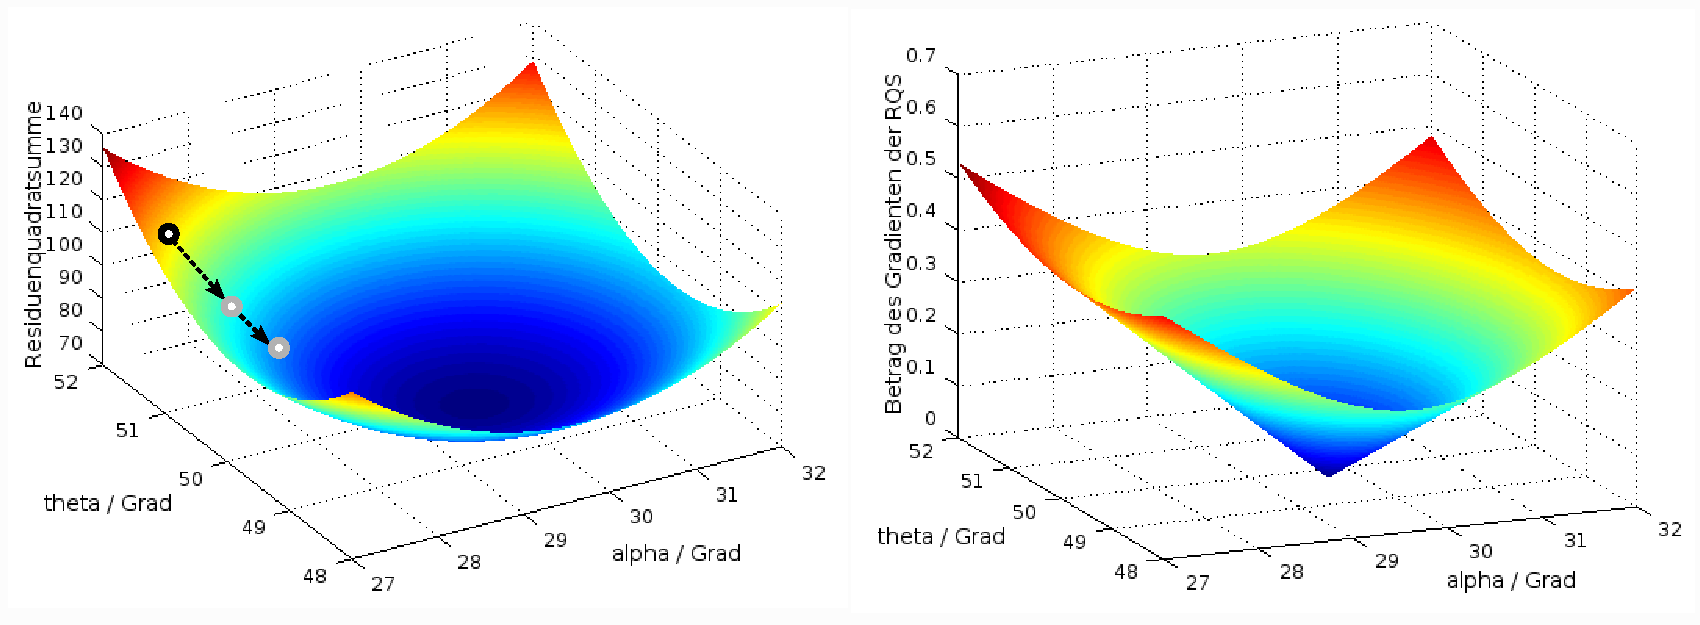
\includegraphics[width=0.95\textwidth, angle = 0]{03_vorlesung/media/LSopti_example1_LS_Grad.pdf}
\end{center}
\caption{Residuenquadratsumme des Beispielmodells mit 2 zu schätzenden Parametern
und Gradienten eingezeichnet als Pfeile (\textsl{links}) und Beträge der
Gradienten als Funktion der 2 zu schätzenden Parameter (\textsl{rechts}).\label{LSoptiExample1Grad}}
\end{figure}
Für zu minimierende Zielfunktionale wie wir sie bei normalverteilten Residuen, also bei
den rundlichen, stetig differenzierbaren Kostenfunktionen als Residuenquadratsummen haben, können wir Verfahren
einsetzen, die nicht nur die Kostenfunktion $Q$ direkt, sondern auch deren Gradienten $\nabla Q$ verwenden.
Hierzu wird \textsl{ein} Startwertetupel (nicht wie bei der Simplexmethode $M+1$)
für die Modellparameter gebracht. Es wird der Gradient, also die Richtung des steilsten
Abhangs der Kostenfunktion zusammen mit dem Wert der Steigung an der Position des Startwerttupels
bestimmt. Dieses Verfahren beleuchten wir im folgenden Abschnitt anhand unseres Beispiels etwas genauer.

\section{Gradientenverfahren für nichtlineare Zielfunktionale}

Das Gradientenverfahren braucht wie alle anderen Methoden zur Schätzung von Parametern, die
nicht linear in die Residuen eingehen, ein Tupel von Startwerten der Parameter, was wir in
Abb.~\ref{LSoptiExample1Grad} als schwarz umrandeten weißen Punkt dargestellt haben.
In Abb.~\ref{LSoptiExample1Grad} ist die Idee illustriert, wie sich die Position des
Parametervektors verändert. Die Änderungsvektoren $\Delta \mathbf{p}$ werden aus der Richtung
des steilsten Abhangs ermittelt, wie durch die Pfeile mit gestrichtelter Linie skizziert. 
Der Gradient des Betrags eines Residuums an der Stelle des Startwertevektors $(\alpha_0, \theta_0)$
ist der Vektor der partiellen Ableitungen
\begin{equation}
\left. \nabla_{\alpha,\theta} \varepsilon_j \right|_{\alpha_0, \theta_0} \; = \;
\left(\begin{array}{c}
\frac{\partial}{\partial \alpha} \\
\frac{\partial}{\partial \theta}
\end{array}\right) \left. \varepsilon_j \right|_{\alpha_0, \theta_0} .
\end{equation}
Das auf die Spitze gestellte Dreieck heißt Nablaoperator.
Die Schreibweise $|_{\alpha_0, \theta_0}$ lesen wir \glqq an der Stelle\grqq ~$(\alpha_0, \theta_0)$.
Für die Minimierung bestimmen wir die Stelle $(\hat \alpha, \hat \theta)$, an der sich die Talsohle
der Mulde der RQS-Funktion befinden. Anders gesagt suchen wir die Position im Modellparameterraum,
die unten in der Mulde RQS-Funktion liegt,
in der keine Steigung mehr vorhanden ist, d.h.\ der Gradient ein Nullvektor ist, d.h.
\begin{equation}
\lim_{\alpha \rightarrow \hat \alpha, \theta \rightarrow \hat \theta} 
\left\{\nabla_{\alpha,\theta} \,
\sum\limits_{j=1}^J \, \varepsilon(\alpha,\theta)_j^2
\right\} \; = \; 
\left(\begin{array}{c}
0 \\
0
\end{array}\right) .
\label{LSschaetzung1}
\end{equation}
Hierbei müssen wir uns aber darüber im Klaren sein, dass Gradient gleich Nullvektor nicht nur
bei einem Minimum vorliegt, sondern auch bei einem Maximum und bei einem Sattelpunkt, weshalb wir
im letzten Abschnitt ein Verfahren kurz vorstellen, das sich mit dieser Problematik besser
auseinander setzt.

Wir ziehen den Nablaoperator in die Summe rein und
verwenden die Kettenregel, äußere Ableitung mal innere Ableitung:
\begin{equation}
\nabla_{\alpha,\theta} \,
\sum\limits_{j=1}^J \, \varepsilon(\alpha,\theta)_j^2
 \; = \; 
\sum\limits_{j=1}^J \, \nabla_{\alpha,\theta} \, \varepsilon(\alpha,\theta)_j^2
 \; = \; 
2 \, \sum\limits_{j=1}^J \, \varepsilon(\alpha,\theta)_j \nabla_{\alpha,\theta} \, \varepsilon(\alpha,\theta)_j
 \; \overset{!}{=} \; 
\left(\begin{array}{c}
0 \\
0
\end{array}\right) .
\label{GradientQ2params}
\end{equation}

Die beiden Parameter $\alpha,\theta$ fassen wir zusammen in einen Parametervektor $\mathbf{p}$ und
betrachten im folgenden den Allgemeinfall für $M$ Parameter $\mathbf{p} = (P_1,\dots,P_M)^\mathsf{T}$.
Die Residuen sind dann jeweils Funktion des Parametervektors
$\boldsymbol \varepsilon(\mathbf{p}) = (\varepsilon_1(\mathbf{p}), \dots, \varepsilon_J(\mathbf{p}))^\mathsf{T}$,
so dass die Kostenfunktion $Q$ entsprechend Funktion des Parametervektors ist
\begin{equation}
Q(\mathbf{p}) \; = \; \boldsymbol \varepsilon^\mathsf{T}(\mathbf{p}) \, \boldsymbol \varepsilon(\mathbf{p}),
\label{Zielfunktional}
\end{equation}
für die wir das Minimum suchen mit
\begin{equation}
\min_{\mathbf{p}} \left\{ Q(\mathbf{p}) \right\}
\end{equation}
indem wir nach dem Nullstellenvektor der Gradientenfunktion
\begin{equation}
\nabla_{\mathbf{p}} Q(\mathbf{p}) \; = \;
 2 \, \boldsymbol \varepsilon^\mathsf{T} \, \left( \nabla_{\mathbf{p}}^\mathsf{T} \boldsymbol \varepsilon \right)
\label{ZielfunktionalGrad}
\end{equation}
suchen, für den $Q$ ein Minimum und nicht ein Maximum oder Sattelpunkt annimmt.
Dabei ist $\nabla_{\mathbf{p}}$ Spaltenvektor und $\nabla_{\mathbf{p}}^\mathsf{T}$ Zeilenvektor
mit den partiellen Ableitungsoperatoren $\frac{\partial}{\partial P_m}$.
Wir suchen dasjenige $\mathbf{p}$ für das
\begin{equation}
\lim_{\mathbf{p} \rightarrow \mathbf{\hat p}}
\nabla_{\mathbf{p}} Q(\mathbf{p}) \; = \; \left(\begin{array}{c} 0\\ \vdots \\ 0 \end{array}\right)
\label{ZielfunktionalGrad1}
\end{equation}
Bei der Suche nach dem Minimum wird mit einem Tupel von Parametern angefangen, also
mit einem Startwertvektor $\mathbf{p}_0$. Dann wird ein Schrittvektor $\Delta \mathbf{p}_0$ ermittelt,
der gegangen wird, um
zu einem Nachfolgepunkt im Raum der Modellparamter zu gelangen $\mathbf{p}_1 = \mathbf{p}_0 + \Delta \mathbf{p}_0$.
Dies erfolgt solange, bis der Parametervektor beliebig dicht an das Minimum von $Q$ gelangt sind. Es gibt damit eine
gewisse Anzahl $K$ von Iterationschritten, derart dass der Vektor $\mathbf{p}_K = \mathbf{\hat p}$ für minimales
$Q$ als Tupel von Schätzwerten für die Modellparameter verwendet wird.
Die einzelnen Iterationsschritte $\kappa$ bedeuten eine Revision des Modellparametervektors
\begin{equation}
\mathbf{p}_\kappa = \mathbf{p}_{\kappa-1} + \Delta \mathbf{p}_{\kappa-1}
\label{Revisionsschritt}
\end{equation}
mittels \textsl{Inkrementvektoren}
$\Delta \mathbf{p}_1, \dots, \Delta \mathbf{p}_{\kappa}, \dots, \Delta \mathbf{p}_{K-1}$.

Wir nehmen eine Taylorreihenentwicklung vor, über die wir die Gradientenfunktion des Zielfunktionals
als lineare Funktion eines \textsl{Inkrementvektors} $\Delta \mathbf{p}$ darstellen. Dazu entwickeln
wir die Residuen $\varepsilon_j$ in Taylorreihe bis zum linearen Term
\begin{equation}
\left(\begin{array}{c}
\varepsilon_1(\mathbf{p}) \\
\vdots \\
\varepsilon_j(\mathbf{p}) \\
\vdots \\
\varepsilon_J(\mathbf{p}) 
\end{array}\right)
\; = \; 
\left(\begin{array}{c}
\varepsilon_1(\mathbf{p}_\kappa) \; + \; \nabla_{\mathbf{p}} \left. \varepsilon_1 \right|_{\mathbf{p}_\kappa} \cdot \Delta \mathbf{p}\\
\vdots \\
\varepsilon_j(\mathbf{p}_\kappa) \; + \; \nabla_{\mathbf{p}} \left. \varepsilon_j \right|_{\mathbf{p}_\kappa} \cdot \Delta \mathbf{p}\\
\vdots \\
\varepsilon_J(\mathbf{p}_\kappa) \; + \; \nabla_{\mathbf{p}} \left. \varepsilon_J \right|_{\mathbf{p}_\kappa} \cdot \Delta \mathbf{p}
\end{array}\right).
\label{TaylorResi1}
\end{equation}
Hier bilden die partiellen Ableitungen der einzelnen Residuen nach allen Parametern eine $J \times M$-Matrix, die \textsl{Jakobimatrix}
genannt wird:
\begin{equation}
\boldsymbol{J}^{(\kappa)} \; = \; \left(\begin{array}{ccc}
\left. \frac{\partial \varepsilon_1}{\partial P_1} \right|_{\mathbf{p}_\kappa} & \dots & \left. \frac{\partial \varepsilon_1}{\partial P_M} \right|_{\mathbf{p}_\kappa} \\
 & \ddots & \\
\left. \frac{\partial \varepsilon_J}{\partial P_1}\right|_{\mathbf{p}_\kappa} & \dots & \left. \frac{\partial \varepsilon_J}{\partial P_M}\right|_{\mathbf{p}_\kappa}
\end{array}\right) .
\end{equation}
Der hochgestellte und in Klammern gesetzte Index $\kappa$ 
an dem Symbol für die \textsl{Jacobimatrix}, soll bedeuten,
dass dies die \textsl{Jacobimatrix} für den Parametervektor an der Stelle
$\mathbf{p}_\kappa$ ist, also für die Position der Modellparameter beim $\kappa$-ten Interationsschritt.
Der Begriff Jacobimatrix bedeutet nur, dass es
sich um eine Matrix partieller Ableitungen handelt.
\begin{quote}
Die \textsl{Jacobimatrix} (benannt nach Carl Gustav Jacob Jacobi; auch 
\textsl{Funktionalmatrix}, \textsl{Ableitungsmatrix} oder \textsl{Jacobische} genannt)
einer differenzierbaren Funktion
$f\colon I \! \! R^{n} \mapsto I \! \! R ^{m}$ ist die 
$m\times n$-Matrix sämtlicher erster partieller Ableitungen.
\end{quote}


Einsetzen dieser Jacobimatrix in Gl.~(\ref{TaylorResi1}) liefert dann
\begin{equation}
\left(\begin{array}{c}
\varepsilon_1(\mathbf{p}) \\
\vdots \\
\varepsilon_J(\mathbf{p}) 
\end{array}\right)
\; = \; 
\left(\begin{array}{c}
\varepsilon_1(\mathbf{p}_\kappa) \\
\vdots \\
\varepsilon_J(\mathbf{p}_\kappa)
\end{array}\right)
\; + \; \boldsymbol{J}^{(\kappa)} \Delta \mathbf{p} .
\label{TaylorResi2}
\end{equation}
Wir schreiben Gl.~(\ref{TaylorResi2}) in Vektorschreibweise, mit $\boldsymbol{\varepsilon}$ hier als Spaltenvektor
der einzelnen Residuen.
\begin{equation}
\boldsymbol{\varepsilon}(\mathbf{p})
\; = \; 
\boldsymbol{\varepsilon}(\mathbf{p}_\kappa)
\; + \; \boldsymbol{J}^{(\kappa)} \Delta \mathbf{p} .
\label{TaylorResi3}
\end{equation}
Ferner setzen wir die Jacobimatrix in Gl.~(\ref{ZielfunktionalGrad}) ein
\begin{equation}
\frac{1}{2} \nabla_{\mathbf{p}} Q(\mathbf{p})  \; = \; \boldsymbol{\varepsilon}^\textsf{T}(\mathbf{p})
 \, \boldsymbol{J}
\label{ZielfunktionalGradJ}
\end{equation}
% \; \overset{!}{=} \; \left(\begin{array}{c} 0\\ \vdots \\ 0 \end{array}\right)
% \label{GradientQv}
Wir setzen die Reihenentwicklung der Residuen Gl.~(\ref{TaylorResi3}) ein und 
den Gradienten Gl.~(\ref{ZielfunktionalGradJ}) in Gl.~(\ref{ZielfunktionalGrad1}) ein.
So erhalten wir ein in $\Delta \mathbf{p}$ lineares Gleichungssystem:
\begin{equation}
\left( \boldsymbol{\varepsilon}(\mathbf{p}_\kappa)
\; + \; \boldsymbol{J}^{(\kappa)} \Delta \mathbf{p}_\kappa \right)^\textsf{T} \, \boldsymbol{J}^{(\kappa)}
\; \overset{!}{=} \; \left( 0 \dots  0 \right)
\label{GradientQlinGl1}
\end{equation}
wobei hier der Nullvektor wie der transponierte Modellparametervektor ein
Zeilenvektor im $I \! \! R^{M}$ ist.
Wir formen diese Gleichung, die in Zeilenvektorschreibweise ist, um in
\begin{equation}
\left( \boldsymbol{J}^{(\kappa)} \Delta \mathbf{p}_\kappa \right)^\textsf{T} \, \boldsymbol{J}^{(\kappa)}
\; \overset{!}{=} \; 
- \boldsymbol{\varepsilon}(\mathbf{p}_\kappa)^\textsf{T} \, \boldsymbol{J}^{(\kappa)}
\label{GradientQlinGl2}
\end{equation}
und transponieren diese, um sie als lineares Gleichungssytem mit Spaltenvektoren vorliegen zu haben
d.h.
\begin{equation}
 \boldsymbol{J}^{(\kappa) \textsf{T}} \, \boldsymbol{J}^{(\kappa)} \, \Delta \mathbf{p}_\kappa
\; \overset{!}{=} \; 
-  \boldsymbol{J}^{(\kappa) \textsf{T}} \, \boldsymbol{\varepsilon}(\mathbf{p}_\kappa) .
\label{GradientQlinGl3}
\end{equation}
Die Lösung dieses linearen Gleichungssystems liefert den Inkrementvektor $\Delta \mathbf{p}_\kappa$,
mit dem wir den Schritt zur nächsten Position $\mathbf{p}_{\kappa+1} \; = \; \mathbf{p}_{\kappa} \, + \,
\Delta \mathbf{p}_{\kappa}$ gehen. Die Iterationen enden, wenn der Betrag der Gradientenfunktion oder
das Quadrat nahe Null, also kleiner als eine sehr kleine Zahl $\epsilon$ ist:
\begin{equation}
 \boldsymbol{\varepsilon}(\mathbf{p}_\kappa)^\mathsf{T}
\, \boldsymbol{J}^{(\kappa)} \, \boldsymbol{J}^{(\kappa) \textsf{T}} \, \boldsymbol{\varepsilon}(\mathbf{p}_\kappa) \;
< \; \epsilon
\end{equation}

Für Kostenfunktionen, die wie in Abb.~\ref{LSoptiExample1Grad}, ein sauber ausgeprägtes Minimum
haben, und für die ein Startwerttupel zu den Modellparametern, das nah genug an der Mulde dran ist und
sehr weit weg von irgendwelchen Maxima und Sattelpunkten, lässt sich auf diese Weise das Minimum
finden.


Um eine sinnvolle Konvergenz zu erzielen, ist eine gute Vorkenntnis, also ein geeignetes 
Modellparametertupel $\mathbf{p}_0$ erforderlich, das in einigen Problemstellungen
nur schwerlich, oder gar nicht verfügbar ist. Das bedeutet, dass nicht klar ist, ob
der Gradient dazu führt, dass der Parametervektor in eine Mulde hinab klettert, oder auf
einen Berggipfel oder entlang eines Sattelpunktes spaziert.

Die Numeriker haben Verfahren entwickelt, die auf dieser Grundidee den Gradienten
der Zielfunktion (Summe der Quadrate der Residuen) zu berechnen
basieren, aber ausgereiferter sind hinsichtlich Stabilität und Konvergenz.
Der sog.\ der \textsl{Levenberg-Marquardt}-Algorithmus ist eine solche gradientenbasierte Methode,
die in den Numerikbibliotheken zu Matlab, Gnu-Octave, Python bis hin zu Labview, für nichtlineare
Regression zur Verfügung gestellt wird. Die Grundidee dieser Methode wollen wir im Folgenden
skizzieren.

\section{Levenberg-Marquardt-Verfahren}
\begin{figure}
\begin{center}
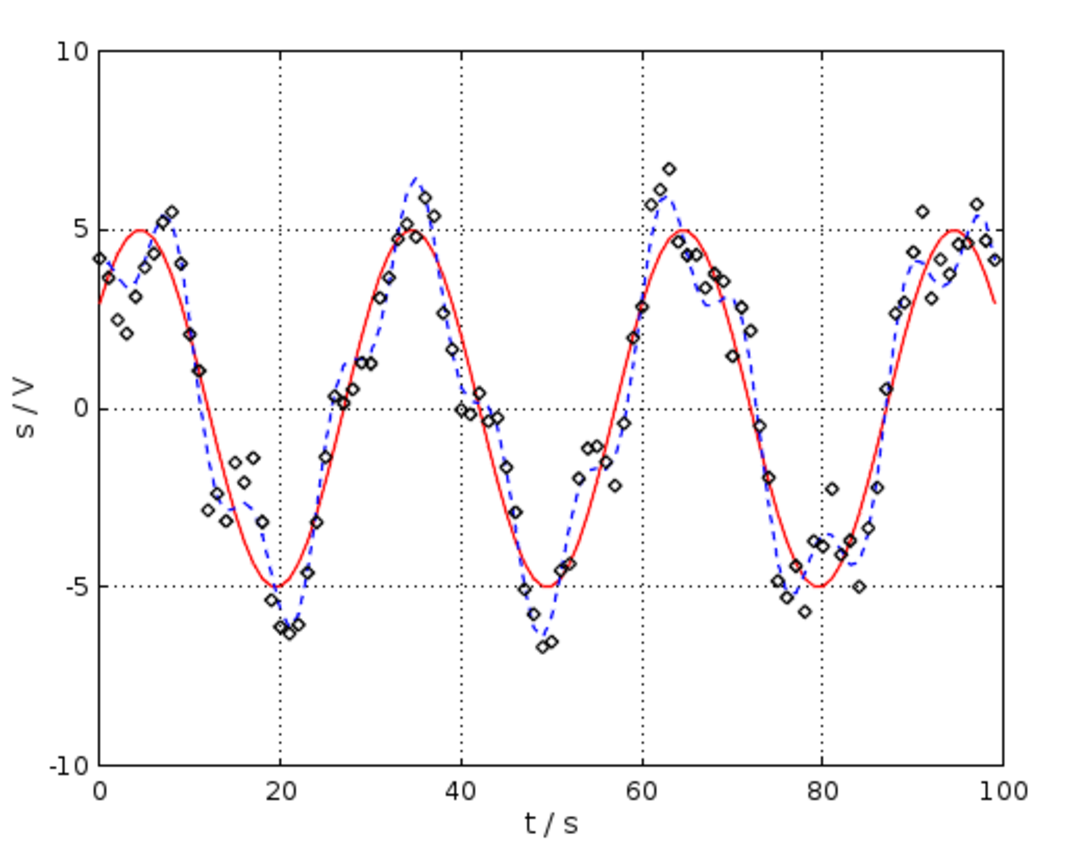
\includegraphics[width=0.6\textwidth, angle = 0]{03_vorlesung/media/pltSS_nonlin_leastsquare_sin_zB1signal.pdf}
\end{center}
\caption{Beispiel eines sinusförmigen Signals.\label{LSoptiExampleSinus}}
\end{figure}
\begin{figure}
\begin{center}
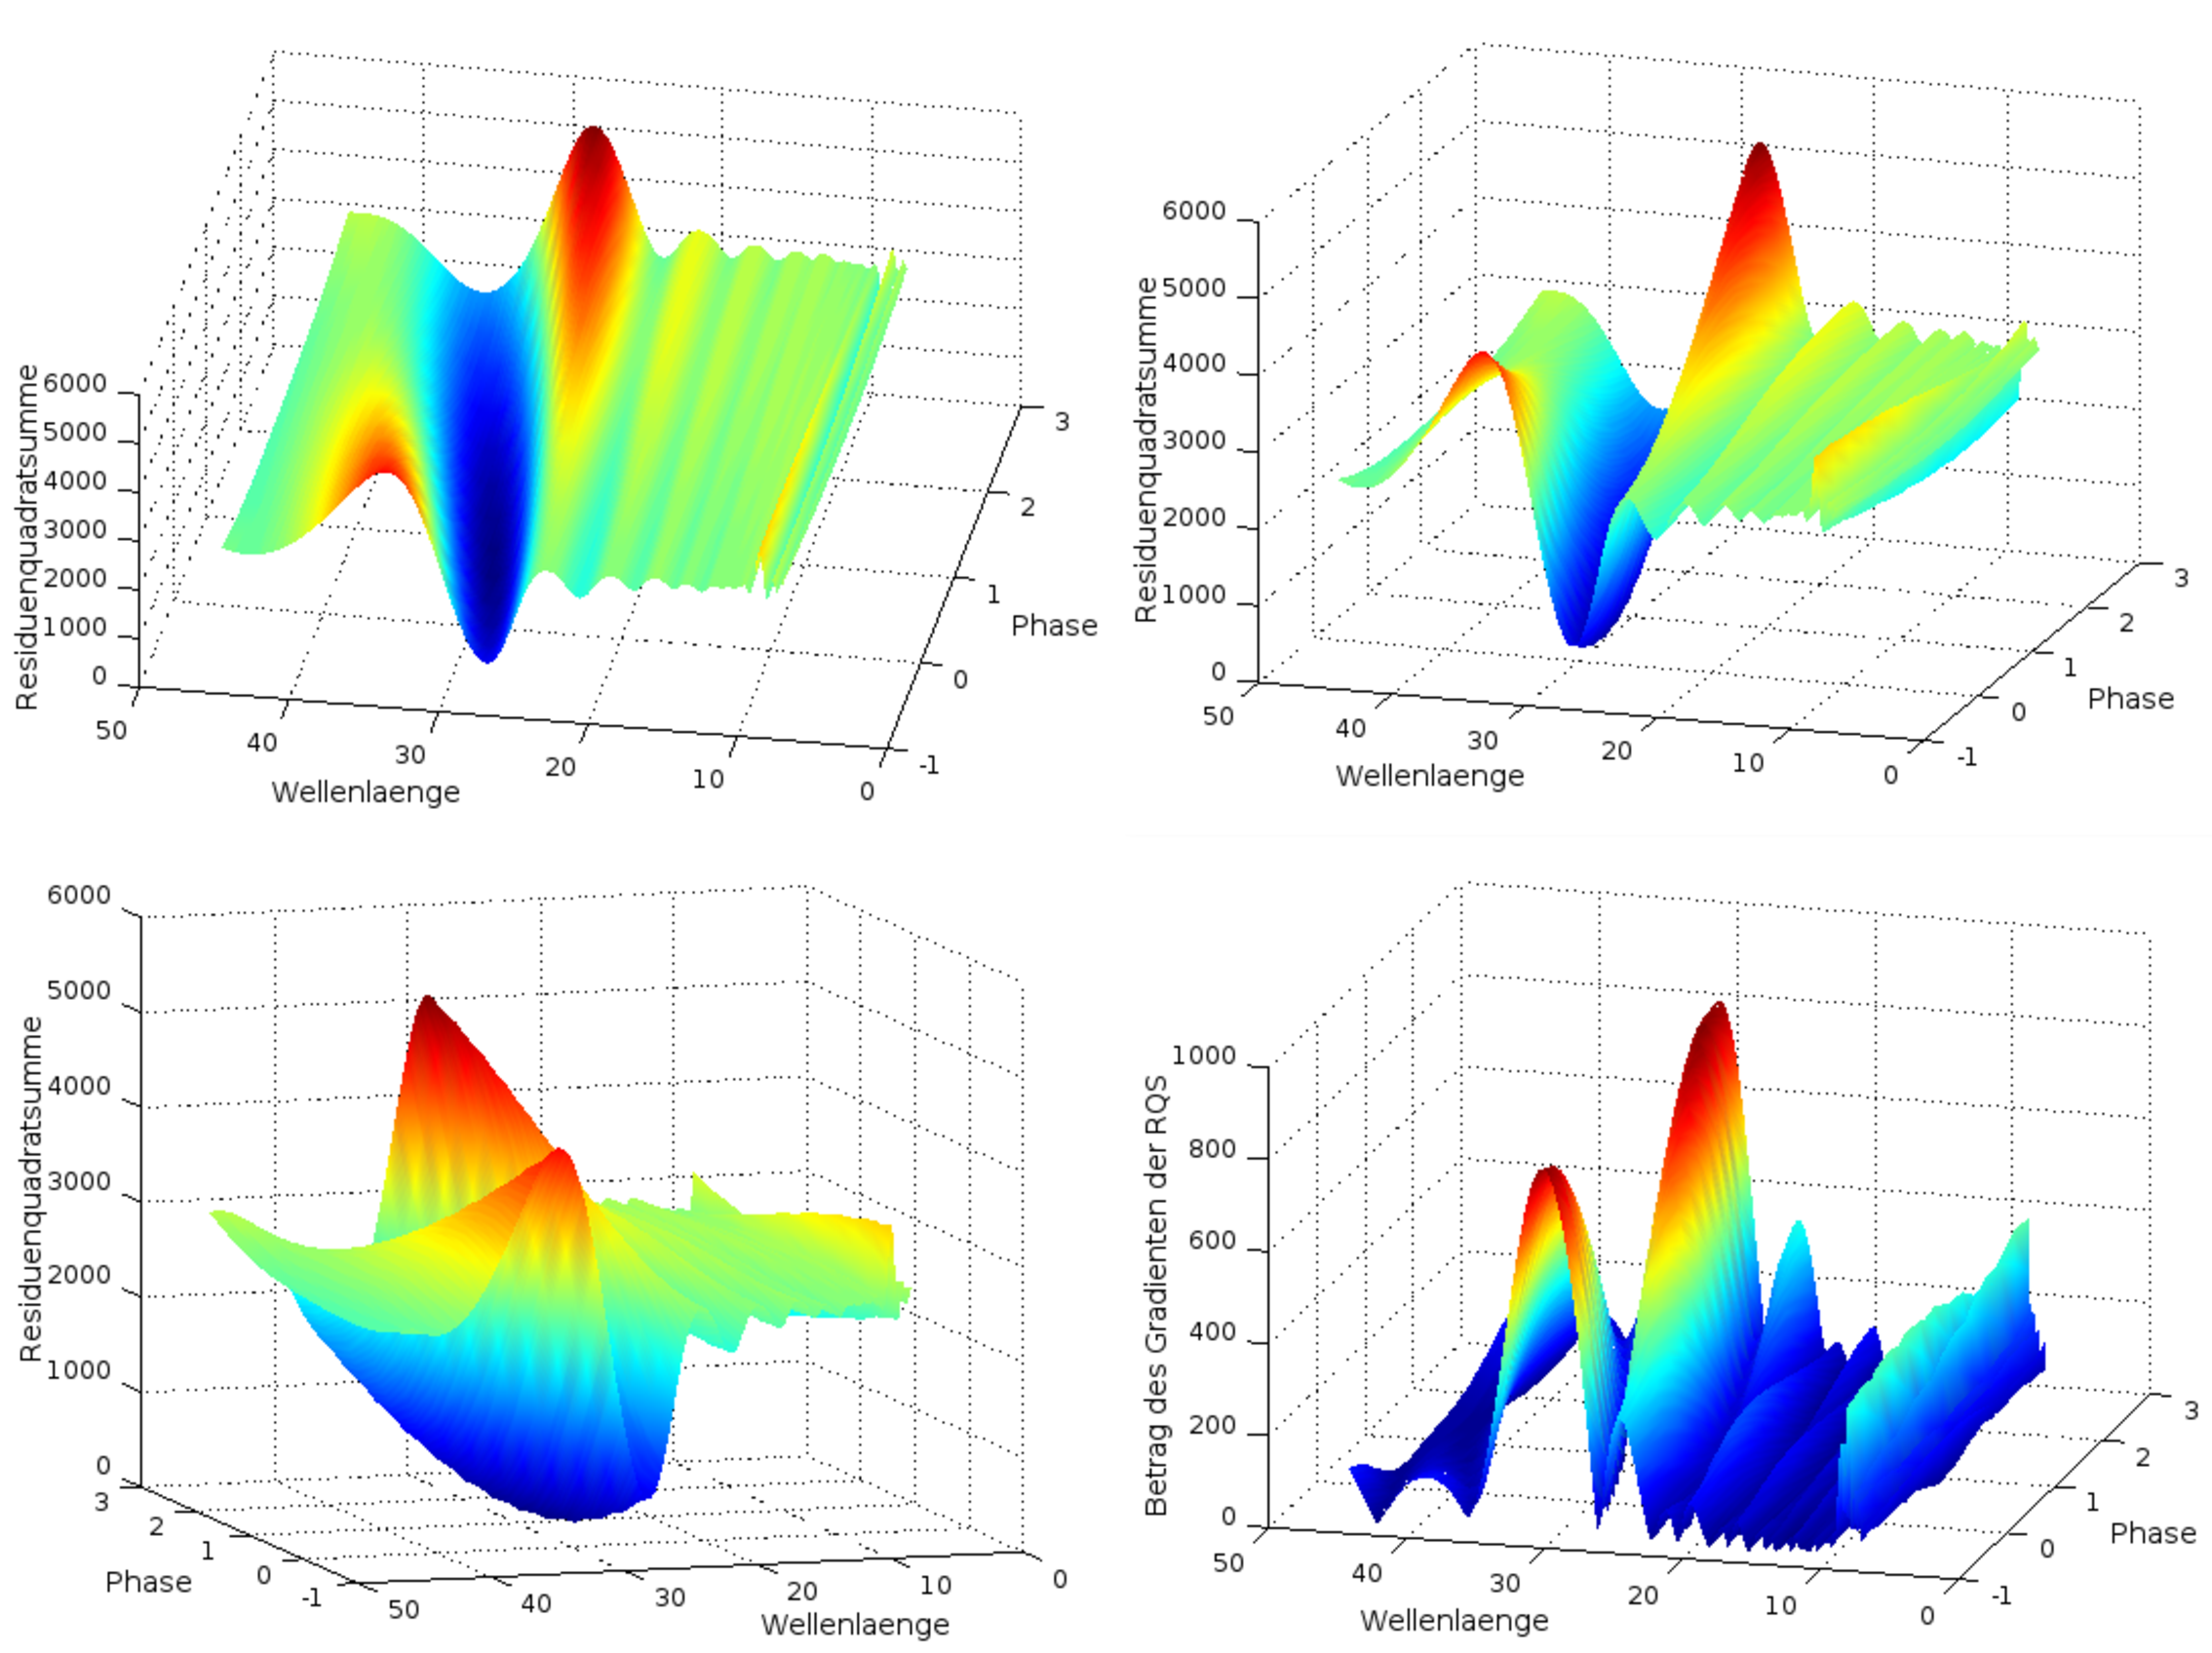
\includegraphics[width=0.9\textwidth, angle = 0]{03_vorlesung/media/pltSS_nonlin_leastsquare_sin_zB1RQS.pdf}
\end{center}
\caption{Residuenquadratsumme des Beispielmodells eines sinusförmigen Signals
in drei verschiedenen Perspektiven dargestellt (\textsl{oben} und \textsl{unten links})
 und die Beträge der
Gradienten als Funktion der 2 zu schätzenden Parameter (\textsl{unten rechts}).\label{LSoptiExample1SinusRQS}}
\end{figure}
Die Problematik, dass sich der Vektor $\Delta \mathbf{p}_{\kappa}$, den wir im
Folgenden \textsl{Inkrementvektor} nennen, verirrt und auf
einen Berggipfel oder entlang eines Sattelpunktes spaziert, soll anhand eines Beispielsignals
illustriert werden. Das Beispiel ist ein zeitabhängiges Spannungssignal mit sinusförmigem Verlauf,
dem als Störung zum einen ein Signal mit höherer Frequenz und kleinerer Amplitude aufmoduliert ist
und zum anderen ein normalverteiltes weißes Rauschen.
Die Amplitude von $5 \, V$ sei fest vorgegeben, aber die zu schätzenden Modellparameter seien
die Wellenlänge und die Phasenlage des Signals. Abb.~\ref{LSoptiExampleSinus} zeigt das Signal als
schwarze Rauten und in Rot das gesuchte \glqq wahre\grqq ~Signal und als blaue, gestrichelte Kurve
das Signal superponiert mit der höherfrequenten Modulation.

Abb.~\ref{LSoptiExample1SinusRQS} zeigt die Summe der Quadrate der Residuen RQS als
Kostenfunktion in drei verschiedenen Ansichten, die zeigen, dass es eine ausgeprägte Minimumsmulde gibt,
aber ebenso ein ausgeprägtes Maximum und noch kleine Rippeln als Nebenminima und Nebenmaxima.
Das Diagramm unten rechts zeigt die Betragsfunktion des Gradienten mit den vielen Nullstellen.
Hier sehen wir, dass sowohl die Maxima als auch die Minima die Nullstellen bilden.

Der \textsl{Levenberg-Marquardt}-Algorithmus ist ein Gradientenverfahren, bei dem das lineare
Gleichungssystems (\ref{GradientQlinGl3}) 
durch Einführen eines Dämpfungsterms erweitert wird. Der Dämpfungsterm stellt einen
Schrittweitenfaktor dar, der den Inkrementvektor
so modifiziert, dass das Optimierungsverfahren besser konvergiert. Dieser
Algorithmus wurde unabhängig voneinander von Levenberg (1944), Girard (1958), Wynne (1959), 
Morrison (1960) und Marquardt (1963) vorgeschlagen. In der Literatur wird heutzutage meist vom 
Levenberg-Marquardt-Algorithmus gesprochen.

Wir schreiben hier nochmal zusammen das zu minimierende Zielfunktional $Q$ aus Gl.~(\ref{ZielfunktionalGrad}) links
und die in Taylorreihe entwickelten Residuen $\boldsymbol{\varepsilon}(\mathbf{p})$
(Gl.~\ref{TaylorResi3}) auf
$$
Q \; = \; \boldsymbol{\varepsilon}(\mathbf{p})^\mathsf{T} \, \boldsymbol{\varepsilon}(\mathbf{p})
\qquad
\boldsymbol{\varepsilon}(\mathbf{p})
\; = \; 
\boldsymbol{\varepsilon}(\mathbf{p}_\kappa)
\; + \; \boldsymbol{J}^{(\kappa)} \Delta \mathbf{p}
$$
und setzen diese ineinander ein, so dass die Kostenfunktion wie folgt aussieht
\begin{equation}
Q \; = \; \left( \boldsymbol{\varepsilon}(\mathbf{p}_\kappa)
\; + \; \boldsymbol{J}^{(\kappa)} \Delta \mathbf{p} \right)^\mathsf{T} \,
\left( \boldsymbol{\varepsilon}(\mathbf{p}_\kappa)
\; + \; \boldsymbol{J}^{(\kappa)} \Delta \mathbf{p} \right) .
\label{ZielfunktionalTaylorResi}
\end{equation}
Damit hatten wir im vorigen Abschnitt einen Ansatz erhalten, der
ein bezüglich des Inkrementvektors $\Delta \mathbf{p}_\kappa$ lineares Gleichungssystem
geliefert hatte. Wir notieren Gl.~(\ref{GradientQlinGl3}) hier noch einmal
\begin{equation*}
 \boldsymbol{J}^{(\kappa) \textsf{T}} \, \boldsymbol{J}^{(\kappa)} \, \Delta \mathbf{p}_\kappa
\; \overset{!}{=} \; 
-  \boldsymbol{J}^{(\kappa) \textsf{T}} \, \boldsymbol{\varepsilon}(\mathbf{p}_\kappa) .
\end{equation*}

Nun modifizieren wir das Gleichungssystem durch Hinzufügen eines Dämpfungsterms
wie folgt
\begin{equation}
\left(
\boldsymbol{J}^{(\kappa) \textsf{T}} \, \boldsymbol{J}^{(\kappa)}
 + \mu \, \mathrm{diag}\left(\boldsymbol{J}^{(\kappa) \textsf{T}} \, \boldsymbol{J}^{(\kappa)}\right)
 \right) \Delta \mathbf{p}_\kappa \;
\overset{!}{=} \; - \boldsymbol{J}^{(\kappa)^\textsf{T}} \, \boldsymbol{\varepsilon}(\mathbf{p}_\kappa)
\label{ZielfunktionalGradTaylorResiDaempf}
\end{equation}
wobei $\mathrm{diag}\left(\boldsymbol{J}^{(\kappa) \textsf{T}} \, \boldsymbol{J}^{(\kappa)}\right)$ 
eine Diagonalmatrix ist, die aus den Matrixelementen auf der Hauptdiagonalen von
$\boldsymbol{J}^{(\kappa) \textsf{T}} \, \boldsymbol{J}^{(\kappa)}$ besteht und die 
Nebendiagonalelemente alle mit Null besetzt hat.

Der Parameter $\mu$ wird Dämpfungsparameter oder \textsl{Marquardtparameter} genannt.
Die Dämpf\-ungs\-strategie besteht darin, dass für große Werte von $\mu$ die Länge
$\sqrt{\Delta \mathbf{p}_\kappa^\mathsf{T} \, \Delta \mathbf{p}_\kappa}$
der Inkrementschritte $\Delta \mathbf{p}_\kappa$ entsprechend verringert wird.

Diese Methode, die  Länge des Inkrementvektors 
$\Delta \mathbf{p}_\kappa$ zu verbessern, also die Werte für den
Dämpf\-ungs\-parameter $\mu$ zu wählen, ist heuristisch.
Es gibt eine Vielzahl von Methoden und Möglichkeiten und wir gucken uns
eine davon an, um einen Einblick zu erhalten, wie soetwas aussehen kann.

Es wird eine Prüfgröße $\rho_{\mu}$ definiert, bei der die Differenz der
Kostenfunktion $Q$ für unterschiedliche Modellparametertupel 
verglichen wird mit der Differenz der die Kostenfunktion an der Nachfolgerstelle
zu dem entsprechenden Punkt auf der approximierenden Tangentialebenen
\begin{equation}
\rho_{\mu} :=\frac{Q(\mathbf{p}_\kappa) - 
Q(\mathbf{p}_\kappa + \Delta \mathbf{p}_\kappa)}
{Q(\mathbf{p}_\kappa) - 
\left( \boldsymbol \varepsilon (\mathbf{p}_\kappa) 
    + \mathbf{J}^{(\kappa)} \Delta \mathbf{p}_\kappa \right)^\mathsf{T}
\left( \boldsymbol \varepsilon (\mathbf{p}_\kappa) 
    + \mathbf{J}^{(\kappa)} \Delta \mathbf{p}_\kappa \right)  } 
=:  \frac{\Delta R(\mathbf{p}_\kappa, \Delta \mathbf{p}_\kappa)}{\Delta \tilde{R}(\mathbf{p}_\kappa, \Delta \mathbf{p}_\kappa)} .
\label{DaempfTuning}
\end{equation}
Die Prüfgröße $\rho_{\mu}$ ist das Verhältnis 
\begin{itemize}
\item der Differenz $\Delta R$ des Zielfunktionals $Q$ zwischen
der Vorgängerposition $\mathbf{p}_\kappa$ und $Q$ an der Nachfolgerposition
$\mathbf{p}_\kappa + \Delta \mathbf{p}_\kappa$
des Parametervektors 
\item relativ zu der Differenz $\Delta \tilde{R}$ zwischen dem $Q$ an der
Stelle der Vorgängerposition $\mathbf{p}_\kappa$ und dem Wert der Residuenquadratsumme
an der Position auf der Tangentialfläche die an der
Stelle $\mathbf{p}_\kappa$ an die Kostenfunktion $Q$ angelegt wird,
\end{itemize}
um dort das Zielfunktional zu approximieren.

Jetzt wird noch eine Vergleichsgröße, ein Schwellwert gebraucht, mit der die
Prüfgröße verglichen wird, oder auch mehrere Schwellwerte. Hier stellen wir
eine Methode vor, bei der zwei Schwellwerte $\beta_0, \beta_1$ als
Ent\-scheid\-ungs\-grund\-lage für die Wahl des
Wertes $\mu$ verwendet werden, um den Inkrementvektor geeignet zu manipulieren.
Für diese beiden heuristischen Schwell\-wert\-para\-meter $\beta_0$, $\beta_1$ 
können wir beispielsweise die Werte $\beta_0 = 0.2$, $\beta_1 = 0.8$ wählen.

Tabelle 1: Entscheidungen zur Behandlung des Marquadtparameters

\begin{tabular}{ll}
\hline\hline
$\rho_{\mu} \le \beta_0 $: &
$\Delta \mathbf{p}_\kappa$ wird nicht akzeptiert \textsl{Gewährleistung der Konvergenz} \\
 & $\mu$ wird vergrößert, z.B.\ durch Verdoppeln  $\mu \rightarrow 2 \mu$,\\
 & und die neue zugehörige Korrektur $\Delta \mathbf{p}_\kappa$ wird berechnet\\
\hline
$\beta_0 < \rho_{\mu} < \beta_1$: & $\Delta \mathbf{p}_\kappa$ wird akzeptiert \\
 & bei der Berechnung von $\Delta \mathbf{p}_{\kappa+1}$
  wird als Anfangswert dasselbe $\mu$ gewählt \\ 
\hline
$\rho_{\mu} \ge \beta_1$: & $\Delta \mathbf{p}_\kappa$ wird akzeptiert \textsl{Effektivität}\\
 & bei der Berechnung  von $\Delta \mathbf{p}_\kappa$ wird \\ 
 & als Anfangswert ein kleinerer Wert für $\mu$ gewählt, z.B.\ durch Halbieren $\mu / 2$ \\
\hline\hline
\end{tabular}

Diese Methode wurde hier auf das zuvor beschriebene Beispiel des in Abb.~\ref{LSoptiExampleSinus}
dargestellten sinusförmigen Signals mit folgendem Gnu-Octave/Matlab-Skript ausprobiert:
\begin{verbatim}
function fit_sin_LMAC(gen_new)
  if gen_new
    t = [0:99]'; % Sekunden
    N = length(t);
%
    a = 5; % Volt
    lam = 30; % Sekunden
    sigma = 0.13*a;
    phi = 0.2*pi;
%
    am = 0.3*a;
    phim = 0.7*pi;
    lamm = 0.3*lam;
%
    st = a*sin(2*pi*t/lam + phi);
    smod = st + am*sin(2*pi*t/lamm + phim);
    s = smod + sigma*randn(1,N);
    save('pltSS_nonlin_leastsquare_sin_zB2.dat','t','s','sigma','a');
  else
    load('pltSS_nonlin_leastsquare_sin_zB1.dat');
  end
%
% Startwerte geraten
%
  p0 = [34; 0.23*pi];
  x = [t(:) s(:)];
%
% Residuen, muessen als Spaltenvektor vorliegen
%
  epsi = @(x, p) (x(:,2) - a*sin(2*pi*x(:,1)/p(1) + p(2)));
%
% partielle Ableitungen der Residuen epsi
% muss M Spalten und J Zeilen haben, wobei M die Anzahl der Fitparameter
% und J die Anzahl der Messpunkte ist
%
  Jac  = @(x, p) [(4*a*pi/p(1)^2)*x(:,1).*cos(2*pi*x(:,1)/p(1)+p(2)).* ...
      (x(:,2)-a*sin(2*pi*x(:,1)/p(1)+p(2))) , ...
      -2*a*cos(2*pi*x(:,1)/p(1)+p(2)).* ...
      (x(:,2)-a*sin(2*pi*x(:,1)/p(1)+p(2))) ];
%
  maxit = 1000; % Anzahl der Iterationen
  tol = 1E-15; % Abbruchbedingung
  beta0 = 0.2;
  beta1 = 0.8;
%
% Startwert des Marquardtparameters
%
  mu0 = 100;
%
% Optimierungsrechnung
%
  p1 = levenberg_marquardt(epsi,Jac,x,p0,mu0,beta0,beta1,maxit,tol);
%
% Ergebnisausgabe
%
  fprintf(stdout,'gefittete Werte: lambda = %1.2f  phi/pi = %1.2f\n', ...
  p1(1), p1(2)/pi );
  sf = @(x, p) a*sin(2*pi*x/p(1) + p(2));
  figure(1);
  plot( t, s, 'kd', ...
    t, st, 'g-;soll;', 'linewidth', 3, ...
    t, sf(t,p0), 'b-.;Startwerte;', 'linewidth', 2,...
    t, sf(t,p1), 'r--;gefittet;', 'linewidth', 2);
  xlabel('t / s','fontsize', 14);
  ylabel('s / V','fontsize', 14);
  set(gca,'fontsize',12);
  grid on;
  print(1,'pltSS_nonlin_leastsquare_sin_zB1.svg','-dsvg');
end
%
function p = levenberg_marquardt(F,DF,x,p0,mu0,beta0,beta1,maxit,tol)
  k = 0;
  mu= mu0;
  p = p0;
  gradQabs = abbruchkrit(F,DF,x,p);
  sflag = 1;
  while (gradQabs>tol) && (k<maxit) && (mu>tol) && (sflag<2)
    [s,mu,sflag] = korrektur(F,DF,x,p,mu,beta0,beta1,tol);
    if sflag==1
      p=p+s;
    end
    gradQabs = abbruchkrit(F,DF,x,p);
    k=k+1;
  end
  fprintf(stdout,'Anzahl Interationen: %d\n', k);
end
%
function [s,mu,sflag] = korrektur(F,DF,x,p,mu,beta0,beta1,tol)
  s = Delta_p(F,DF,x,p,mu);
  Q = F(x,p)'*F(x,p);
  DR = Q - F(x,p+s)'*F(x,p+s);
  DRtilde = Q - (F(x,p)+DF(x,p)*s)'*(F(x,p)+DF(x,p)*s);
   sflag = 1;
  if DRtilde > tol
    if DR <= beta0*DRtilde
      sflag = 0;
      mu    = 2*mu;
    elseif DR >= beta1*DRtilde
      mu    = mu/2;
    end
  else
    sflag = 2;
  end
end
%
function s = Delta_p(F,DF,x,p,mu)
  JTJ = DF(x,p)'*DF(x,p);
  s = -( JTJ + mu*diag(JTJ) )\(DF(x,p)'*F(x,p));
end
%
function gradQabs = abbruchkrit(F,DF,x,p)
  gradQabs = ( F(x,p)'*DF(x,p) * DF(x,p)'*F(x,p) );
end
\end{verbatim}

Dieses Gnu-Octave-Skript hat dazu das in Abb.~\ref{LSoptiExampleSinusFitted}
dargestellte Ergebnis mit den Werten
\begin{verbatim}
Anzahl Interationen: 62
gefittete Werte: lambda = 30.20  phi/pi = 0.22
\end{verbatim}
geliefert.
\begin{figure}
\begin{center}
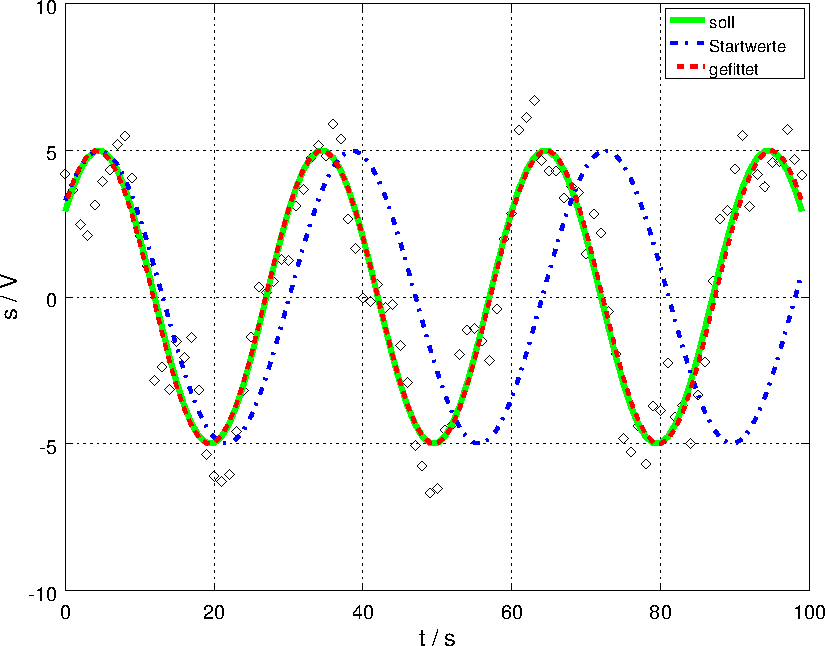
\includegraphics[width=0.6\textwidth, angle = 0]{03_vorlesung/media/pltSS_nonlin_leastsquare_sin_zB1.pdf}
\end{center}
\caption{Beispiel eines sinusförmigen Signals mit Levenberg-Marquadt-Fit gemäß
Gln.~(\ref{ZielfunktionalGradTaylorResiDaempf}) und (\ref{DaempfTuning}) zusammen mit
den Entscheidungen aus Tabelle 1.\label{LSoptiExampleSinusFitted}}
\end{figure}

Dieses Beispiel hat einen Modellansatz
\begin{equation}
s(t) \; = \; a \sin(2\pi \frac{t}{\lambda} + \varphi) \; + \; \varepsilon \qquad 
\textrm{mit} \qquad \varepsilon \sim {\cal N}(0,\sigma) 
\end{equation}
bei dem die Residuen in Richtung von $s$ streuen und bei dem die Abtastpunkte
entlang der Zeitachse $t$ als Regressor vorgegeben sind, so dass
wir einen Regressionsansatz der Gestalt
\begin{equation}
\epsilon_j \; = \; Y_j \; - \; f(X_j, \boldsymbol{\theta}) \qquad \textrm{mit} \qquad 
j=1, 2,\dots, J 
\end{equation}
vorliegen haben. Die Kostenfunktion sieht damit wie folgt aus
\begin{equation}
Q \; = \; \sum\limits_{j=1}^J \left(Y_j \; - \; f(X_j, \boldsymbol{\theta})\right)^2.
\end{equation}
Für die nichtlineare Regression gibt es in Gnu-Octave und Matlab beispielsweise folgende
Funktion:
\begin{verbatim}
[f, p, cvg, iter] =leasqr (x, y, init, F);
\end{verbatim}
Angewendet auf unser Beispiel vom sinusförmigen Signal kann sie in folgender Weise
verwendet werden
\begin{verbatim}
function fit_sin(gen_new)
  load('pltSS_nonlin_leastsquare_sin_zB1.dat');
  p0 = [34; 0.23*pi];
  sf = @(x, p) a*sin(2*pi*x/p(1) + p(2));
  [f1, p1, kvg1, iter1, corp1, covp1, covr1, stdresid1, Z1, r21] = ...
    leasqr (t(:), s(:), p0, sf);
  fprintf(stdout,'gefittete Werte: lambda = %1.2f  phi/pi = %1.2f\n', ...
    p1(1), p1(2)/pi );
  figure(1);
  plot( t, s, 'kd', ...
    t, st, 'g-.;soll;', ...
    t, sf(t,p0), 'b--;Startwerte;', ...
    t, sf(t,p1), 'r-;gefittet;');
  xlabel('t / s','fontsize', 14);
  ylabel('s / V','fontsize', 14);
  set(gca,'fontsize',12);
  grid on;
end
\end{verbatim}
und wir erhalten folgendes Ergebnis
\begin{verbatim}
gefittete Werte: lambda = 29.91  phi/pi = 0.18
\end{verbatim}

\section{Gradientenverfahren mit unterschiedlichen Varianzen}
\label{unterschiedVar}

Die Varianzen (und Kovarianzen) der Residuen sind immer auch Funktion der Modellparameter. Als wir die
Maximum-Likelihood-Methode eingeführt haben, hatten wir sie ausgeklammert und bei der Bestimmung
des Minimums über die Summer der kleinsten Residuenquadrate weggekürzt. Sie
lassen sich für den Fall ausklammern, bei dem die Streuung bezüglich des Modells
für alle Messpunkte gleich ist, also
\begin{equation}
Q(\mathbf{p}) \; = \;
 \frac{\boldsymbol{\varepsilon}(\mathbf{p})^\mathsf{T} \, \boldsymbol{\varepsilon}(\mathbf{p})}{\sigma^2(\mathbf{p}))}
\end{equation}
und
\begin{equation}
\nabla_{\mathbf{p}} Q(\mathbf{p})  \; = \; 
\frac{2}{\sigma^2(\mathbf{p})} \boldsymbol{\varepsilon}^\textsf{T}(\mathbf{p})
 \, \boldsymbol{J} \overset{!}{=} \; \left(\begin{array}{ccc} 0 & \dots & 0 \end{array}\right)
\label{ZielfunktionalGradJmitSigma}
\end{equation}
was einfach mit $\frac{\sigma^2(\mathbf{p})}{2}$ multipliziert werden kann, so dass wir mit
den Residuen wie oben beschreiben weiter arbeiten können, indem wir diese in Taylorreihe entwickeln.

Für den Fall, dass es unterschiedliche Varianzen für Residuen der verschiedenen Beobachtungstupel
$(X_{1,j},\dots,X_{N,j})$ gibt, ordnen wir $\sqrt{\sigma_j^2} = \sigma_j$ 
den Residuen zu mit
\begin{equation}
Q(\mathbf{p}) \; = \;
  \left(\begin{array}{ccc}
  \frac{\varepsilon_1(\mathbf{p})}{\sigma_1(\mathbf{p})} & \dots &
 \frac{\varepsilon_J(\mathbf{p})}{\sigma_J(\mathbf{p})} \end{array} \right)
\, \left(\begin{array}{c} \frac{\varepsilon_1(\mathbf{p})}{\sigma_1(\mathbf{p})}\\
 \vdots\\ \frac{\varepsilon_J(\mathbf{p})}{\sigma_J(\mathbf{p})}\end{array} \right)
\label{ZielfunktionalJmitW}
\end{equation}
d.h.\ kurz ohne jedesmal das \glqq Funktion von $\mathbf{p}$\grqq oder
\glqq abhängig von $\mathbf{p}$\grqq, also $(\mathbf{p})$,
mitzuschreiben
\begin{equation}
Q(\mathbf{p}) \; = \;
  \boldsymbol{\varepsilon}^\textsf{T}
\, \left(\begin{array}{cccc} \frac{1}{\sigma_1^2} & \dots & & 0 \\
  & \ddots & \\
 0 & & \dots &  \frac{1}{\sigma_J^2} \end{array} \right) \, \boldsymbol{\varepsilon}
\label{ZielfunktionalJmitW1}
\end{equation}
Je stärker eine Beobachtung $j$ abweicht, also je größer die Varianz $\sigma_j^2$,
desto geringer fällt der Summand $\frac{\varepsilon_j^2}{\sigma_j^2}$ in der Kostenfunktion $Q$
ins Gewicht, weshalb man diese auch als Gewichte $w_j = \frac{1}{\sigma_j^2}$ bezeichnet
und die Matrix als Gewichtsmatrix $\mathbf{W}$ also
\begin{equation}
Q(\mathbf{p}) \; = \;
  \boldsymbol{\varepsilon}^\textsf{T}
\, \mathbf{W} \, \boldsymbol{\varepsilon}
\label{ZielfunktionalJmitW2}
\end{equation}
und mit
\begin{equation}
\frac{1}{2} \nabla_{\mathbf{p}} Q(\mathbf{p})  \; = \; \boldsymbol{\varepsilon}^\textsf{T}(\mathbf{p})
 \, \mathbf{W} \, \boldsymbol{J}
\label{ZielfunktionalGradJW}
\end{equation}
sieht unser Optimierungsproblem wie folgt aus
\begin{equation}
\lim_{\mathbf{p} \rightarrow \mathbf{\hat p}}
\boldsymbol{\varepsilon}^\textsf{T}(\mathbf{p})
 \, \mathbf{W}(\mathbf{p}) \, \boldsymbol{J}(\mathbf{p})
 \; = \; \left(\begin{array}{ccc} 0 & \dots & 0 \end{array}\right) .
\label{ZielfunktionalGrad1W}
\end{equation}
Die Gleichungen (\ref{GradientQlinGl3}) und (\ref{ZielfunktionalGradTaylorResiDaempf})
werden damit zu
\begin{equation}
 \boldsymbol{J}^{(\kappa) \textsf{T}} \, \mathbf{W}(\mathbf{p}_\kappa) \, 
\boldsymbol{J}^{(\kappa)} \, \Delta \mathbf{p}_\kappa
\; \overset{!}{=} \; 
-  \boldsymbol{J}^{(\kappa) \textsf{T}} \, \mathbf{W}(\mathbf{p}_\kappa) \, 
\boldsymbol{\varepsilon}(\mathbf{p}_\kappa) .
\label{GradientQlinGl3W}
\end{equation}
und mit Dämpfungs- bzw.\ Marquardtparameter
\begin{equation}
\left(
\boldsymbol{J}^{(\kappa) \textsf{T}} \, \mathbf{W}(\mathbf{p}_\kappa) \, \boldsymbol{J}^{(\kappa)}
 + \mu \, \mathrm{diag}(\boldsymbol{J}^{(\kappa) \textsf{T}} \, \mathbf{W}(\mathbf{p}_\kappa) \, \boldsymbol{J}^{(\kappa)}) \right) \Delta \mathbf{p}_\kappa \;
\overset{!}{=} \; - \boldsymbol{J}^{(\kappa)^\textsf{T}} \, 
\mathbf{W}(\mathbf{p}_\kappa) \, \boldsymbol{\varepsilon}(\mathbf{p}_\kappa) .
\label{ZielfunktionalGradTaylorResiDaempfW}
\end{equation}

Es gibt aber auch Fragestellungen mit unterschiedlichen Varianzen $\sigma_i^2$ 
zu den direkten Messgrößen $X_i$. Ein Beispiel dafür
\begin{figure}
\begin{center}
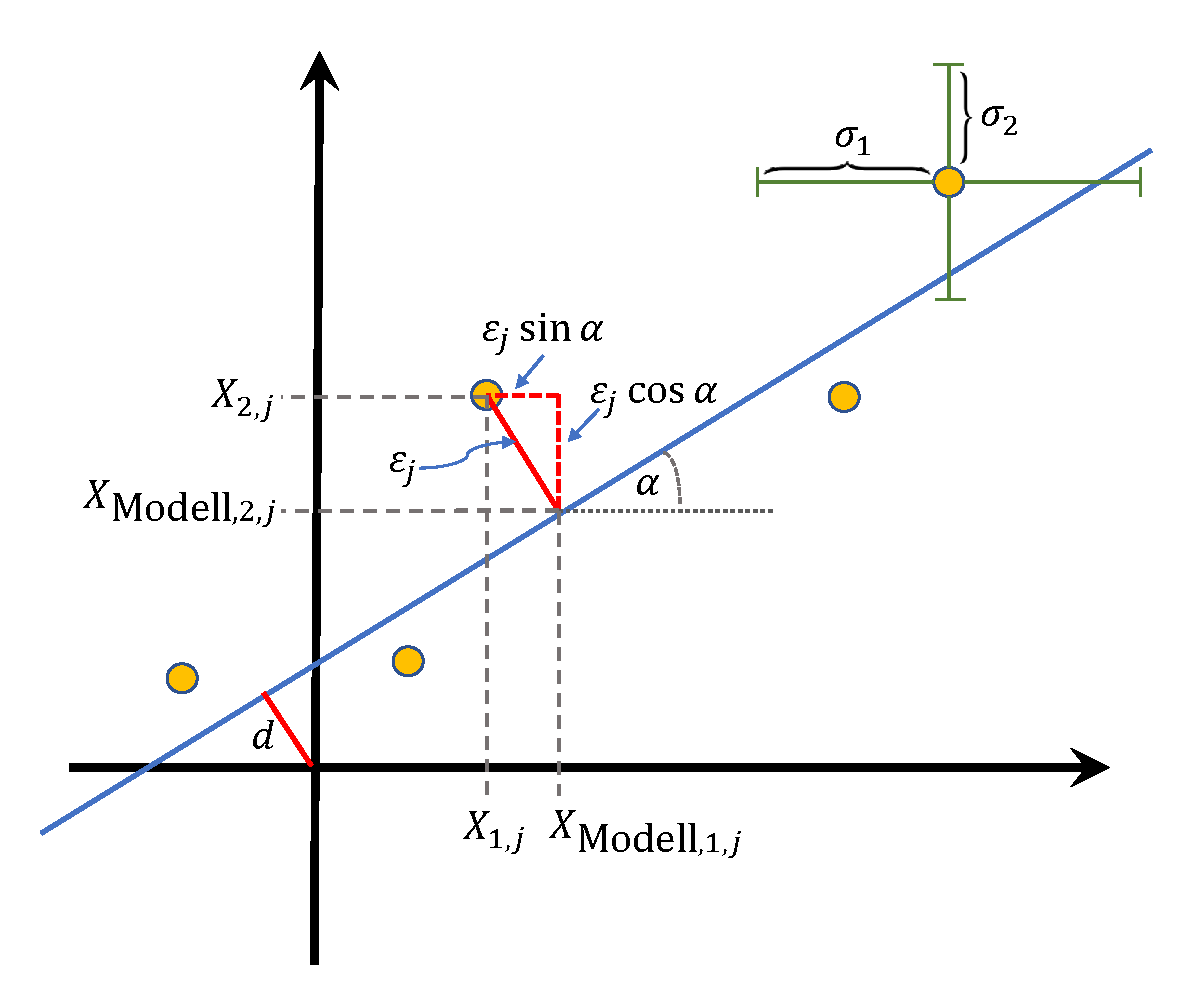
\includegraphics[width=100mm]{03_vorlesung/media/ResiduenVarianzen.pdf}
\end{center}
\caption{Veranschaulichung für Schätzung von Geradenparametern durch
Minimierung der Summe der Quadrate der Residuen bei verschiedenen Varianzen 
$\sigma_1^2$ und $\sigma_2^2$ der beiden direkten Messgrößen $X_1$ und $X_2$
\label{ResiduenVarianzen}}
\end{figure}
ist eine Gerade in einer Ebene mit den Modellparametern $\alpha$ für den Winkel und
$d$ für den Abstand der Geraden vom Koordinatenursprung
\begin{equation}
\varepsilon_j \; = \; 
\left(\begin{array}{c} X_{1,j}\\ X_{2,j}\end{array}\right) \cdot
\left(\begin{array}{c} -\sin(\alpha)\\ \cos(\alpha)\end{array}\right) \; - \; d .
\label{TLSgerade}
\end{equation}
Hier stehen die Residuen $\varepsilon_j$ des $j$-ten Messpunktes $(X_{1,j}, X_{2,j})$ 
senkrecht auf der Modellgeraden, siehe Abb.~\ref{ResiduenVarianzen}, weil beide
Messgrößen $X_1$ und $X_2$ gleichermaßen Zufallsgrößen sind und nicht eine davon
ein Regressor ist die andere ein Regressand ist. Bei dieser \textsl{Least-Square} Methode
spricht man auch von \textsl{Total Least-Square} Methode, weil \glqq total\grqq ~alle Größen
streuen können, also Zufallsgrößen sind.

\begin{equation}
Q(\alpha, d) \; = \;
\sum\limits_{j=1}^J \,  \left(\frac{\varepsilon_j(\alpha, d) \sin(\alpha)}{\sigma_1}\right)^2
\; + \; \sum\limits_{j=1}^J \, \left(\frac{\varepsilon_j(\alpha, d) \cos(\alpha)}{\sigma_2}\right)^2 .
\end{equation}
Hier haben wir also die $\sigma_i^2$ als Varianzen der Abweichungskomponenten
der Messgröße $X_i$ (vektorwertige Residuen!) für alle $j=1,\dots,J$ Beobachtungen
und nicht Varianzen $\sigma_j^2$ für das skalarwertige Residuum der $j$-ten Beobachtung.
Die allgemeine Form mit Kovarianzen sieht dann also so aus
\begin{equation}
Q(\mathbf{p}) \; = \;
 \sum\limits_{j=1}^J \, \vec \varepsilon(X_{1,j},\dots,X_{N,j},\mathbf{p})^\mathsf{T} \, 
\boldsymbol{\Sigma}(X_{1,j},\dots,X_{N,j},\mathbf{p})^{-1} \, \vec \varepsilon(X_{1,j},\dots,X_{N,j},\mathbf{p})_j .
\label{generalLSmethod}
\end{equation}
In diesem Zusammenhang erfolgt die nichtlineare Optimierung, indem nicht
die Residuen in Taylorreihe entwickelt, sondern die Gradientenfunktion $\nabla Q$ direkt.


\section{Robuste Schätzverfahren}
\label{robustEstimation}

Wir haben nun eine Kostenfunktion $Q$ mit Gewichtsfaktoren kennengelernt, Gl.~(\ref{ZielfunktionalJmitW2}),
bei der die Gewichte die Kehrwerte der Varianzen sind $w_j = \frac{1}{\sigma_j^2}$, sich eigentlich
aus der Abweichung der Beobachtungen vom Modell ergeben. Wenn kein {\`a} priori Wissen über
diese Varianzen vorliegt, aber bekannt ist, dass die Verteilung der
Residuen aller Beobachtungen nicht gauß\-ver\-teilt ist, soll das Problem dennoch mit der
Maximum-Likelihood-Methode gelöst werden. Es kommt vor, dass einzelne Beobachtungen
sehr weit von der Erwartung entfernt sind. Man sagt, dass sie signifikant abweichen. Die Gaußverteilung
erlaubt dieses auch, denn sie hat einen Definitionsbereich für die Residuen $\varepsilon$,
der von minus Unendlich bis plus Unendlich geht, ihre Ausläufer auch \textsl{Tails} genannt,
sind unbegrenzt. Die Wahrscheinlichkeit ist aber sehr gering, kleiner als $5~\%$, dass der Betrag der
Residuen $\varepsilon$ einen Wert annimmt, der größer als
$1.65 \, \sigma$ ist, aber er kann auftreten. Liegen deutlich mehr als $5~\%$
der Beobachtungen außerhalb eines Vertrauensintervalls von beispielsweise $[-3 \sigma, 3 \sigma]$,
dann ist dies ein Indiz dafür sein, dass das Modell unzureichend ist. Es kann sein, dass es auch nicht
um ein vollständigeres Modell geht, sondern darum, nur die zum betrachteten Modell passenden Beobachtungen
berücksichtigen zu wollen. Die übrigen Beobachtungen sollen als Ausreißer, die nicht zum
eigentlichen zu untersuchenden Prozess gehören, nicht an dem \textsl{Least-Square-Fit}
beteiligt werden oder zumindest ihre Beteiligung daran (ihr Gewicht) reduziert wird.

Die Idee für die Realisierung dieser Aufgabe ist, die Verteilung der Residuen durch Umgewichten so zu verändern, das
sie wieder die Gestalt einer Normalverteilung bekommt. Wir führen Gewichtsfaktoren $w = \delta$ ein,
die eine Funktion des Abstands $\varepsilon$ einer Beobachtung vom Modell ist, so dass die Wahrscheinlichkeitsdichte 
der Abweichung $\tilde \varepsilon$ einer Normalverteilung folgt. Gesucht ist eine Gewichtsfunktion
$\delta \! : \varepsilon \mapsto \delta(\varepsilon)$ für die gilt
\begin{equation}
\tilde \varepsilon \; = \; \delta(\varepsilon) \; \varepsilon \quad \Rightarrow
\quad \tilde \varepsilon \sim {\cal N}(0,\sigma) .
\end{equation}
Mit Hilfe der Gewichtsfunktion werden aus den Residuen die Gewichtsfaktoren
$w_j = \delta_j = \delta(\varepsilon_j)$ berechnet. Da man die Residuen erst nach
Schätzung der Modellparameter gewinnt, erfordert dies wie bei der nichtlinearen Optimierung
auch sonst, einen iterativen Prozess.

Wir betrachten folgende Kostenfunktion
\begin{equation}
Q(\mathbf{p}) \; = \; \sum_{j=1}^J \, \delta_j \, \varepsilon_j(\mathbf{p})^2 .
\label{robustEstim}
\end{equation}

Zunächst werden die Parameter ungeachtet möglicher Ausreißer mittels \textsl{Least Square}-Methode
ohne Gewichte
\begin{equation}
 \min_{\mathbf{p}} Q(\mathbf{p}) \qquad \mathrm{mit} \qquad 
Q(\mathbf{p}) \; = \; \sum_{j=1}^J \, \varepsilon_j(\mathbf{p})^2 .
\label{linEstim}
\end{equation}
geschätzt mit $\mathbf{p}_0$.

Wir betrachten wieder ein einfaches Beispiel, in dem es nur einen Parameter $y$ gibt und eine 
Messgröße $X_1$ mit $J$ Beobachtungen $(X_{1,1},\dots,X_{1,J})$.
Dabei wird davon ausgegangen, dass die Beobachtungen zu einer Grundgesamtheit, also zu einem Parameter gehören.
Die Beobachtungswerte werden histogrammiert. Das Histogramm ist in Abb.~\ref{biasExampleKap3} dargestellt.
\begin{figure}
\begin{center}
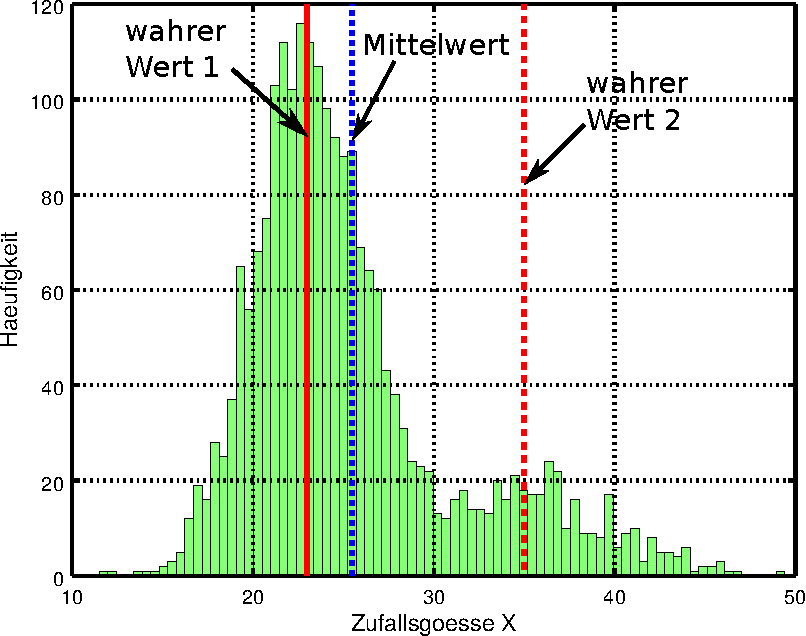
\includegraphics[width=90mm]{03_vorlesung/media/learn_robust.pdf}
\caption{Beispiel für nicht erwartungsgemäße Beobachtungen}
\label{biasExampleKap3}
\end{center}
\end{figure}
Für das Histogramm werden $K \, = \, 80$ Klassen (engl.\ \textsl{bins}) gewählt, die Anzahl der Beobachtungen umfasst $J \, = \, 2200$.
Die Klassenbreite ist dann
\begin{equation}
\Delta \xi \; = \; \frac{1}{K} \left( \max \left\{X_{1,j}\right\} \; - \; \min \left\{X_{1,j}\right\} \right)
\end{equation}
so dass $K+1$ Klassengrenzen $\xi_{\mathrm{G}, k}$ vorliegen,
deren Indizes wir von Null bis $K$ zählen:
\begin{equation}
 \xi_{\mathrm{G}, k} \; = \; k \, \Delta \xi \; + \; \min \left\{X_{1,j}\right\}
\qquad k = 0, \dots, K
\label{limkthbin}
\end{equation}
und die Mitte in der jeweiligen Klasse für den Wert der Klasse verwenden
\begin{equation}
 \xi_k \; = \; k \, \Delta \xi  \, + \, \frac{1}{2} \Delta \xi  \; + \; \min \left\{X_{1,j}\right\}
\qquad k = 1, \dots, K
\label{kthbin}
\end{equation}
wobei die Anzahl der Klassen $K$ ist.

Die Anzahl der Einzelbeobachtungen, für die gilt
\begin{equation}
\xi_{\mathrm{G}, k-1} \; \leq \; X_{1,j} \; <  \xi_{\mathrm{G}, k},
\end{equation}
nennen wir \textsl{Häufigkeit} $n_k$. Bei der letzten Klasse, also für
$k = K$ wird auch bei der rechten Intervallgrenze ein $\leq$.
Damit ist die diskrete Funktion $n(\xi)$ die Häufigkeitsverteilung.

Der Schätzwert für den Parameter ist nach der Maximum-Likelihood / Least-Square-Methode der
Mittelwert, der hier den Wert $25.47$ annimmt. In Wirklichkeit gehören die Beobachtungswerte gar nicht zu
nur einer Grundgesamtheit, sondern $1750$ gehören zu dem Parameter $\mu_1 \, = \, 23.00$ und $450$ zu $\mu_2 \, = \, 35.00$.
Diese Wirklichkeit kennt aber niemand. Bei Betrachten des Histogramms sieht der Messtechniker jedoch, dass ein
Nebenmaximum vorliegt, es keine reine Gaußverteilung ist. Die weiter entfernt liegenden Beobachtungen sollen unterdrückt werden
durch entsprechende Wahl zugehöriger Gewichtsfaktoren $\delta_j$.

Eine mögliche Wahl für die Gewichtsfaktoren ist die \textsl{Tuckey biweight}-Funktion.
\begin{equation}
\delta_j \; = \;
\left\{ \begin{array}{cl}
\left( 1 \, - \, \left( \frac{X_{1,j} \, - \, y^{(\kappa)}}{c^{(\kappa)}} \right)^2 \right)^2 & 
	\mathrm{falls} \; \mid X_{1,j} \, - \, y^{(\kappa)} \mid \, \leq \, c^{(\kappa)} \\
0 & \mathrm{sonst}
\end{array} \right.
\end{equation}
wobei $\kappa$ der Zähler für den Iterationsschritt ist und $c^{(\kappa)}$ ein passend zur Anwendung zu wählender Faktor ist, hier beispielsweise
\begin{equation}
c^{(\kappa)} \; = \; \mathrm{median} \mid X_{1,j} \, - \, y^{(\kappa)} \mid 
\end{equation}
Die Kostenfunktion, deren Gewichte von den iterativ bestimmten Residuen und damit von den
iterativ geschätzten Parametern abhängt, stellt ein nichtlineares Optimierungsproblem
$ \min_{\mathbf{p}} Q(\mathbf{p}) $ dar, mit
\begin{equation}
Q(\mathbf{p}) \; = \; \sum_{j=1}^J \; \varepsilon_j^2 \;
\left( 1 \, - \, \left( \frac{\varepsilon_j(\mathbf{p}) }{c(\mathbf{p})} \right)^2 \right)^2 \;
H(\mid \varepsilon_j(\mathbf{p}) \mid - c(\mathbf{p})) \;
H(c(\mathbf{p}) - \mid \varepsilon_j(\mathbf{p}) \mid ),
\label{robustEstim2}
\end{equation}
wobei $H$ für \textsl{Heaviside}- oder Sprungfunktion steht.

\begin{figure}
\begin{center}
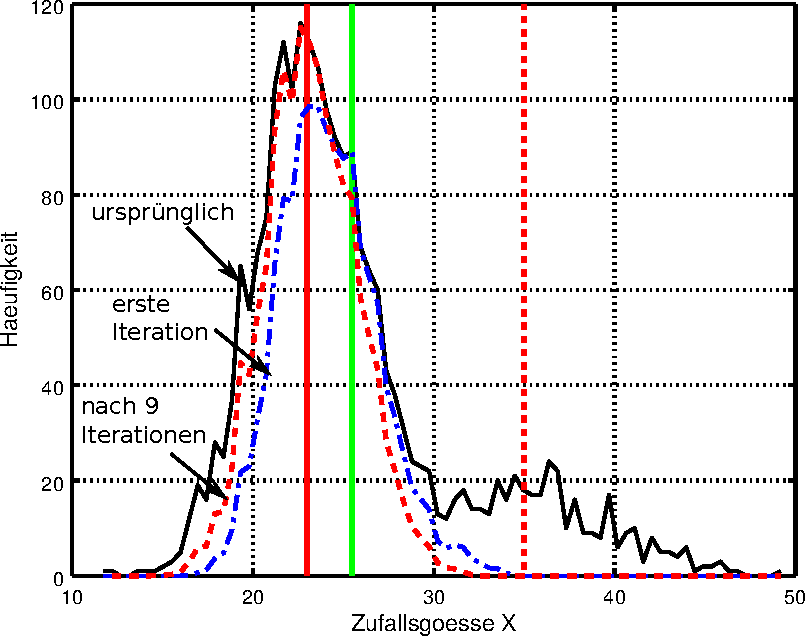
\includegraphics[width=100mm]{03_vorlesung/media/learn_robust_2.pdf}
\caption{\label{RobustIter} Umgewichten um die Verteilungform der Normalverteilung anzupassen}
\end{center}
\end{figure}

Der Median von den Absolutbeträgen der Residuen $\varepsilon_j \, = \, X_{1,j} \, - \, y^{(\kappa)}$ wird dadurch gewonnen,
dass man die Werte der Größe nach sortiert und dann den mittleren nimmt, also den, auf dem Platz in der Mitte der sortierten
Anordnung liegt.
Abb.~\ref{RobustIter} stellt die ursprüngliche Häufigkeitsverteilung aus Abb.~\ref{biasExampleKap3} als
durchgezogene, schwarze Linie dar. Nach dem ersten Iterationsschritt der Umgewichtung, hat sich die Verteilung so verändert,
wie es durch die blaue gestrichpunktete Linie gezeigt wird, zu der ein Mittelwert von $24.20$ gehört. Nach mehr als acht Iterationen
wurde ein Mittelwert von $23.23$ erzielt und die mit rot gestrichelter Verteilungskurve eingezeichnet sind.

